\section{Correspondence Between Models}

\valentin{Gathered some definitions that are scattered and propose a unifying terminology and notation to agree upon}

\begin{definition}\label{def:kmodel}
  A (relational) Kripke model is a triple $\kmodel = \langle \W, {\R}, \V \rangle$ where:
  \begin{enumerate}
    \setlength{\itemsep}{0pt}
    \item $\W$ is a non-empty set of states;
    \item $\R$ is a binary accessibility relation on $\W$;
    \item $\V: \W \to 2^{\props}$ is a valuation function.
  \end{enumerate}
  We use $\W_{\kmodel}$, $\R_{\kmodel}$, and $\V_{\kmodel}$, to indicate $\W$, $\R$, and $\V$, respectively.
  By a pointed Kripke model, we mean a pair $\kmodel,s$ where $\kmodel$ is a Kripke model and $s \in \W_{\kmodel}$.
\end{definition}

% \begin{definition}\label{def:fmorphism}
%   Let $\kmodel_1$ and $\kmodel_2$ be Kripke models.
%   A function $f: \W_{\kmodel_1} \to \W_{\kmodel_2}$ is a homomorphism from $\kmodel_1$ to $\kmodel_2$, written $f: \kmodel_1 \to \kmodel_2$, iff:
%     \begin{enumerate}[label=(\alph*)]
%       \setlength{\itemsep}{0pt}
%       \item $w \R_{\kmodel_1} w'$ implies $f(w) \R_{\kmodel_2} f(w')$;
%       \item $p \in \V_{\kmodel_1}(w)$ implies $p \in \V_{\kmodel_2}(f(w))$.
%     \end{enumerate}
%   % We use $f: \kmodel_1 \to \kmodel_2$ to indicate a relational homomorphism from $\kmodel_1$ to $\kmodel_2$.
% \end{definition}

% % Note that, if we view Kripke models as first-order relational models, then, relational homomorphisms are the well-known homomorphisms of first-order relational models.
% The following proposition is immediate.

% \begin{proposition}
%   Let $f: \kmodel_1 \to \kmodel_2$ and $g: \kmodel_2 \to \kmodel_3$ be relational homomorphisms, whose underlying functions are $f: \W_{\kmodel_1} \to \W_{\kmodel_2}$ and $g: \W_{\kmodel_2} \to \W_{\kmodel_3}$.
%   The composition $(g \circ f): \W_{\kmodel_1} \to \W_{\kmodel_3}$ yields a relational homomorphism $(g \circ f): \kmodel_1 \to \kmodel_3$.
% \end{proposition}

% \begin{definition}\label{def:bisimulation}
%   Let $\kmodel_1$ and $\kmodel_2$ be Kripke models.
%   A bisimulation between $\kmodel_1$ and $\kmodel_2$ is a non-empty binary relation ${\bisim} \subseteq (\W_{\kmodel_1} \times \W_{\kmodel_2})$ s.t.\ for all $s_1 \bisim s_2$:
%     \begin{description}
%       \setlength{\itemsep}{0pt}
%       \item[\textnormal{(atomic harmony)}] $p \in \V_{\kmodel_1}(s_1)$ iff $p \in \V_{\kmodel_2}(s_2)$;
%       \item[\textnormal{(zig/forth)}] $s_1 \R_{\kmodel_1} s_3$ implies there is $s_2 \R_{\kmodel_2} s_4$ s.t.\ $s_2 \bisim s_4$;
%       \item[\textnormal{(zag/back)}] $s_2 \R_{\kmodel_2} s_3$ implies there is $s_1 \R_{\kmodel_1} s_3$ s.t.\ $s_2 \bisim s_4$;
%     \end{description}
%   We use $\kmodel_1, s_1 \bisim \kmodel_2, s_2$ to indicate there is a bisimulation between $\kmodel_1$ and $\kmodel_2$ s.t.\ $s_1 \bisim s_2$.
% \end{definition}

\begin{definition}\label{def:bmodel}
  A bi-relational Kripke model is a tuple $\bmodel = \tuple{\W, {\preccurlyeq}, \R, \V}$ where:
  \begin{enumerate}
    \setlength{\itemsep}{0pt}
    \item $\W$ is a non-empty set of states;
    \item $\preccurlyeq$ is a partial order on $\W$;
    \item $\R$ is a binary accessibility relation on $\W$;
    \item $\V: \props \to 2^{\W}$ is a valuation function.
  \end{enumerate}
  Bi-relational Kripke models further satisfy the following conditions:
  \begin{enumerate}[label=(\alph*)]
    \setlength{\itemsep}{0pt}
    \item for all $t \succcurlyeq s$ and $s \R u$, there is $t \R v$ and $v \succcurlyeq u$;
    \item for all $s \R t$ and $t \preccurlyeq u$, there is $s \preccurlyeq v$ and $v \R u$;
    \item for all $s \preccurlyeq t$, $p \in \V(s)$ implies $p \in \V(t)$.
  \end{enumerate}
  The conditions (a) and (b) above are depicted in \Cref{fig:bframe}.
  If $v$ in (a) and (b) is unique, $\bmodel$ is called \emph{universal}.
  We write $\preccurlyeq^{\equiv}$ and $\R^{\equiv}$ for the equivalence closure of $\preccurlyeq$ and $\R$, respectively.
  We call $\bmodel$ \emph{cartesian} iff whenever $s \preccurlyeq^{\equiv} t$ and $t \R^{\equiv} u$, then, $s = u$.
  We use $\W_{\bmodel}$, $\preccurlyeq_{\bmodel}$, $\R_{\bmodel}$, and $\V_{\bmodel}$, to indicate $\W$, $\preccurlyeq$, $\R$, and $\V$, respectively.
\end{definition}

\begin{figure}[t]
  \centering
  \footnotesize
  \begin{tikzpicture}[modal,node distance = 10mm]
    \node (c) {(a)};
    \node[point] (a) [above left=of c,label=left:$t$] {};
    \node[point] (b) [above right=of c,label=right:$v$] {};
    \node[point] (d) [below left=of c,label=left:$s$] {};
    \node[point] (e) [below right=of c,label=right:$u$] {};
    \path[->] (a) edge[dotted] node[above] {$\R$} (b);
    \path[->] (d) edge node[above] {$\R$} (e);
    \path[->] (d) edge node[left] {$\preccurlyeq$} (a);
    \path[->] (e) edge[dotted] node[right] {$\preccurlyeq$} (b);
  \end{tikzpicture}
  \hspace{1.5cm}
  \begin{tikzpicture}[modal,node distance = 10mm]
    \node (c) {(b)};
    \node[point] (a) [above left=of c,label=left:$v$] {};
    \node[point] (b) [above right=of c,label=right:$u$] {};
    \node[point] (d) [below left=of c,label=left:$s$] {};
    \node[point] (e) [below right=of c,label=right:$t$] {};
    \path[->] (a) edge[dotted] node[above] {$\R$} (b);
    \path[->] (d) edge node[above] {$\R$} (e);
    \path[->] (d) edge[dotted] node[left] {$\preccurlyeq$} (a);
    \path[->] (e) edge node[right] {$\preccurlyeq$} (b);
  \end{tikzpicture}
  \caption{Frame Conditions on Bi-relational Kripke models}
  \label{fig:bframe}
\end{figure}

\begin{definition}\label{def:bsat}
  Let $A$ be a formula, $\bmodel$ be a bi-relational model, and $s \in \W_{\bmodel}$.
  The relation $\bmodel, s \Vdash A$ is defined recursively as:
  \[\begin{array}{lcl}
      \bmodel, s \nVdash \bot \\%& \text{iff} & \text{false} \\
      \bmodel, s \Vdash p & \text{iff} & p \in \V_{\bmodel}(s) \\
      \bmodel, s \Vdash \lnot B & \text{iff} & \text{for all } s \preccurlyeq_{\bmodel} t,~ \bmodel, t \nVdash B \\
      \bmodel, s \Vdash B \land C & \text{iff} & \bmodel, s \Vdash B \text{ and } \bmodel, s \Vdash C \\
      \bmodel, s \Vdash B \lor C & \text{iff} & \bmodel, s \Vdash B \text{ or } \bmodel, s \Vdash C \\
      \bmodel, s \Vdash B \to C & \text{iff} & \text{for all } s \preccurlyeq_{\bmodel} t,~ \bmodel, t \Vdash B \text{ implies } \bmodel, t \Vdash C \\
      \bmodel, s \Vdash \Diamond B & \text{iff} & \text{exists } s \R_{\bmodel} t \text{ s.t.\ } \bmodel, t \Vdash B \\
      \bmodel, s \Vdash \Box B & \text{iff} & \text{for all } s \preccurlyeq_{\bmodel} t \text{ and } t \R_{\bmodel} u,~ \bmodel, u \Vdash B
  \end{array}\]
  We write $\bmodel \Vdash A$ iff $\bmodel, s \Vdash A$ for all $s \in \W_{\bmodel}$.
  Moreover, we write $\Vdash A$, and call $A$ a tautology, iff $\bmodel \Vdash A$ for all bi-relational Kripke models $\bmodel$.
\end{definition}

\begin{definition}\label{def:imodel}
  A hierarchical model is a tuple $\hmodel = \tuple{\kmodels, \preccurlyeq}$ where:
  \begin{enumerate}
    \setlength{\itemsep}{0pt}
    \item $\kmodels$ is a non-empty set of Kripke models;
    \item $\preccurlyeq$ is a preorder on $\kmodels$.
  \end{enumerate}
  Hierarchical models further satisfy the following constraints for all $\kmodel_1 \preccurlyeq \kmodel_2$:
  \begin{enumerate}[label=(\alph*)]
    \setlength{\itemsep}{0pt}
    \item ${\W_{\kmodel_1} \subseteq \W_{\kmodel_2}}$;
    \item ${\R_{\kmodel_1} \subseteq \R_{\kmodel_2}}$;
    \item for all $w \in \W_{\kmodel_1}$, $\V_{\kmodel_1}(w) \subseteq \V_{\kmodel_2}(w)$.
  \end{enumerate}
  We use $\kmodels_{\hmodel}$, and $\preccurlyeq_{\hmodel}$, to indicate $\kmodels$, and $\preccurlyeq$, respectively.
\end{definition}

\begin{proposition}
  If $\bmodel$ is a hierarchical model, then, $\preccurlyeq_{\bmodel}$ is a partial order.
\end{proposition}
\begin{proof}
  We only need to prove that $\preccurlyeq_{\bmodel}$ is antisymmetric, i.e., if $\kmodel_1 \preccurlyeq_{\bmodel} \kmodel_2$ and $\kmodel_2 \preccurlyeq_{\bmodel} \kmodel_1$, then, $\kmodel_1 = \kmodel_2$.
  The result is immediate from conditions (a)--(c).
\end{proof}

\begin{definition}\label{def:sat:imodel}
  Let $A$ be a formula, $\hmodel$ be a hierarchical model, $\kmodel \in \kmodels_{\hmodel}$, and $s \in \W_{\kmodel}$.
  The relation $\kmodel, s \Vdash^{\hmodel} A$ is defined recursively as:
  \[\begin{array}{lcl}
    \kmodel, s \nVdash^{\hmodel} \bot \\
    \kmodel, s \Vdash^{\hmodel} p & \text{iff} & p \in \V_{\kmodel}(s) \\
    \kmodel, s \Vdash^{\hmodel} \lnot B & \text{iff} & \text{for all } \kmodel \preccurlyeq_{\hmodel} \kmodel',~ \kmodel', s \nVdash^{\hmodel} B \\
    \kmodel, s \Vdash^{\hmodel} B \land C & \text{iff} & \kmodel, s \Vdash^{\hmodel} B \text{ and } \kmodel, s \Vdash^{\hmodel} C \\
    \kmodel, s \Vdash^{\hmodel} B \lor C & \text{iff} & \kmodel, s \Vdash^{\hmodel} B \text{ or } \kmodel, s \Vdash^{\hmodel} C \\
    \kmodel, s \Vdash^{\hmodel} B \to C & \text{iff} & \text{for all } \kmodel \preccurlyeq_{\hmodel} \kmodel',~ \kmodel', s \Vdash^{\hmodel} B \text{ implies } \kmodel', s \Vdash^{\hmodel} C \\
    \kmodel, s \Vdash^{\hmodel} \Diamond B & \text{iff} & \text{exists } s \R_{\kmodel} t \text{ s.t.\ } \kmodel, t \Vdash^{\hmodel} B \\
    \kmodel, s \Vdash^{\hmodel} \Box B & \text{iff} & \text{for all } \kmodel \preccurlyeq_{\hmodel} \kmodel' \text{ and } s \R_{\kmodel'} t,~ \kmodel', t \Vdash^{\hmodel} B
  \end{array}\]
  We write $\kmodel \Vdash^{\hmodel} A$ iff $\kmodel, s \Vdash^{\hmodel} A$ for all $s \in \W_{\kmodel}$.
  Also, we write $\Vdash^{\hmodel} A$ iff $\kmodel \Vdash^{\hmodel} A$ for all $\kmodel \in \kmodels_{\hmodel}$.
  Finally, we write $\Vdash A$, and call $A$ a tautology, iff $\Vdash^{\hmodel} A$ for all hierarchical models $\hmodel$.
\end{definition}

We can map hierarchical models to bi-relational Kripke models in a semantics-preserving way.
This is made precise in~\Cref{def:hs2bks,prop:hs2bks}.

\begin{proposition}[{\cite[Lemma~8.1.2~p.151]{simpson1994}}]\label[proposition]{prop:hs2bks}
  Let $\hmodel$ be a hierarchical model.
  Define $\bmodel_{\hmodel} = \tuple{\W, {\preccurlyeq}, \R, \V}$ where:
  \begin{enumerate}
    \setlength{\itemsep}{0pt}
    \item $\W = \setof{(\kmodel, s)}{ \kmodel \in \kmodels_{\hmodel} \text{ and } s \in \W_{\kmodel}}$;
    \item ${\preccurlyeq} = \setof{ (\bb{s}, \bb{t}) }{ {\bb{s}_1 \preccurlyeq_{\hmodel} \bb{t}_1} \text{ and } {\bb{s}_2 = \bb{t}_2}}$;
    \item $\R = \setof{ (\bb{s}, \bb{t}) }{ \set{\bb{s}_1, \bb{t}_1} \subseteq \kmodels_{\hmodel} \text{ and } {\bb{s}_1 = \bb{t}_1} \text{ and } {\bb{s}_2 \R_{\bb{s}_1} \bb{t}_2}}$;
    \item %$\V_{\hmodel}: \props \to 2^{\S_{\hmodel}}$ is s.t.\
      for all $\bb{s} \in \W$, $\V(\bb{s}) = \V_{\bb{s}_1}(\bb{s}_2)$.
  \end{enumerate}
  It follows that:
  \begin{enumerate}[label=(\alph*)]
    \setlength{\itemsep}{0pt}
    \item $\bmodel_{\hmodel}$ is a universal bi-relational Kripke model; and
    \item $\kmodel, s \Vdash^{\hmodel} A$ iff $\bmodel_{\hmodel}, (\kmodel,s) \Vdash A$.
    \item $\hmodel$ is finite implies $\bmodel_{\hmodel}$ is finite;
  \end{enumerate}
\end{proposition}

In \cite[$\S$~8.1.2]{brauner11}, it is claimed that, in general, bi-relational Kripke models cannot be translated into hierarchical models.
The stated reason is that there are more bi-relational Kripke models than intuitionistic modal models, though no formal justification for this claim is provided.
At the same time, in \cite[p.~152]{simpson1994}, it is shown that cartesian bi-relational Kripke models can be translated into hierarchical models in a semantic preserving way.
\valentin{When we started to look into this problem Carlos messaged Torben about the claim he makes in his book. He replied, but did not provide a good justification for what he says. From the result in Simpson's PhD thesis, I think it should be clear that the translation from cartesian bi-relational Kripke models to hierarchical models cannot preserve finiteness, or cartesian bi-relational Kripke models cannot be used to characterize $\IK$.}

\begin{definition}\label{def:wmodel}
  A weaved model is a tuple $\wmodel = \tuple{\kmodels, \F}$ where:
  \begin{enumerate}
    \setlength{\itemsep}{0pt}
    \item $\kmodels$ is a non-empty set of Kripke models;
    % \item $\preccurlyeq$ is a preorder on $\kmodels$;
    \item $\F$ is a set of homomorphisms on $\kmodels$.
  \end{enumerate}
  Weaved models further satisfy the following constraints:
  \begin{enumerate}[label=(\alph*)]
    \setlength{\itemsep}{0pt}
    \item for all $\kmodel$, the identity homomorphism ${\id_{\kmodel}: {\kmodel \to \kmodel}} \in \F$;
    \item for all $\{{f: {\kmodel_1 \to \kmodel_2}},{g: {\kmodel_2 \to \kmodel_3}}\} \subseteq \F$, ${(g \circ f): {\kmodel_1 \to \kmodel_3}} \in \F$.
  \end{enumerate}
  We use $\kmodels_{\wmodel}$, and $\F_{\wmodel}$, to indicate $\kmodels$, and $\F$, respectively.
\end{definition}

\begin{proposition}\label[proposition]{prop:preorder:wmodel}
  Let $\wmodel$ be a weaved model.
  For all $\{\kmodel_1, \kmodel_2\} \subseteq \kmodels_{\wmodel}$, define $\kmodel_1 \preccurlyeq_{\wmodel} \kmodel_2$ iff there is ${f: \kmodel_1 \to \kmodel_2} \in \F_\wmodel$.
  Then, $\preccurlyeq_{\wmodel}$ is a preorder on $\kmodels_{\wmodel}$.
\end{proposition}

\begin{definition}\label{def:sat:wmodel}
  Let $\wmodel$ be a weaved model, $\kmodel \in \kmodels_{\wmodel}$, $s \in \W_{\kmodel}$, and $A$ be a formula.
  The relation $\kmodel, s \Vdash^{\wmodel} A$ is defined recursively as:
  \[\begin{array}{lcl}
    \kmodel, s \nVdash^{\wmodel} \bot \\
    \kmodel, s \Vdash^{\wmodel} p & \text{iff} & p \in \V_{\kmodel}(s) \\
    \kmodel, s \Vdash^{\wmodel} \lnot B & \text{iff} & \text{for all } {f: \kmodel \to \kmodel'} \in \F_{\wmodel},~ \kmodel', f(s) \nVdash^{\wmodel} B \\
    \kmodel, s \Vdash^{\wmodel} B \land C & \text{iff} & \kmodel, s \Vdash^{\wmodel} B \text{ and } \kmodel, s \Vdash^{\wmodel} C \\
    \kmodel, s \Vdash^{\wmodel} B \lor C & \text{iff} & \kmodel, s \Vdash^{\wmodel} B \text{ or } \kmodel, s \Vdash^{\wmodel} C \\
    \kmodel, s \Vdash^{\wmodel} B \to C & \text{iff} & \text{for all } {f: \kmodel \to \kmodel'} \in \F_{\wmodel},~ \kmodel', f(s) \Vdash^{\wmodel} B \text{ implies } \kmodel', f(s) \Vdash^{\wmodel} C \\
    \kmodel, s \Vdash^{\wmodel} \Diamond B & \text{iff} & \text{exists } s \R_{\kmodel} t \text{ s.t.\ } \kmodel, t \Vdash^{\wmodel} B \\
    \kmodel, s \Vdash^{\wmodel} \Box B & \text{iff} & \text{for all } {f: \kmodel \to \kmodel'} \in \F_{\wmodel},~ f(s) \R_{\kmodel'} t,~ \kmodel', t \Vdash^{\wmodel} B
  \end{array}\]
  We write $\kmodel \Vdash^{\wmodel} A$ iff $\kmodel, s \Vdash^{\wmodel} A$ for all $s \in \W_{\kmodel}$.
  Also, we write $\Vdash^{\wmodel} A$ iff $\kmodel \Vdash^{\wmodel} A$ for all $\kmodel \in \kmodels_{\wmodel}$.
  Finally, we write $\Vdash A$, and call $A$ a tautology, iff $\Vdash^{\wmodel} A$ for all weaved models $\wmodel$.
\end{definition}

%%%%%%%%%%%%%%%%%%%%%%%%%%%

{
\color{blue}
\begin{definition}\label{def:homomorphism}
  A homomorphism from a Kripke model $\kmodel_1$ to a Kripke model $\kmodel_2$ is a function $f: \W_{\kmodel_1} \to \W_{\kmodel_2}$, written $f: \kmodel_1 \to \kmodel_2$, s.t.:
    \begin{description}
      \setlength{\itemsep}{0pt}
      \item[\textnormal{(inclusion)}] $p \in \V_{\kmodel_1}(s)$ implies $p \in \V_{\kmodel_2}(f(s))$;
      \item[\textnormal{(forth)}] $s \R_{\kmodel_1} t$ implies $f(s) \R_{\kmodel_2} f(t)$.
    \end{description}
  A homomorphism from a pointed Kripke model $\kmodel_1, s$ to a pointed Kripke model $\kmodel_2, t$, written $f: \kmodel_1,s \to \kmodel_2, t$, is a homomorphism $f: \kmodel_1 \to \kmodel_2$ s.t.\ $f(s) = t$.
\end{definition}

\begin{proposition}
  Let $\kmodel$ be a Kripke model.
  First, the identity function $\id_{\kmodel}: {\W_{\kmodel} \to \W_{\kmodel}}$ is a homomorphism $\id_{\kmodel}: \kmodel,s \to \kmodel,s$.
  Second, the composition of homomorphisms $f: \kmodel_1,s \to \kmodel_2,t$ and $g: \kmodel_2,t \to \kmodel_3,u$ is a homomorphism $(g \circ f): \kmodel_1,s \to \kmodel_3,u$.
\end{proposition}

\begin{definition}\label{def:wmodel:pointed}
  A weaved model is a tuple $\wmodel = \tuple{\kmodels, \F}$ where:
  \begin{enumerate}
    \setlength{\itemsep}{0pt}
    \item $\kmodels$ is a non-empty set of pointed Kripke models;
    % \item $\preccurlyeq$ is a preorder on $\kmodels$;
    \item $\G$ is a set of homomorphisms on $\kmodels$ closed under identities and composition.
  \end{enumerate}
  We use $\kmodels_{\wmodel}$, and $\F_{\wmodel}$, to indicate $\kmodels$, and $\G$, respectively.
\end{definition}

\begin{proposition}\label[proposition]{prop:preorder:wmodel:pointed}
  Let $\wmodel$ be a weaved model.
  The relation $\kmodel,s \preccurlyeq_{\wmodel} \kmodel',t$ iff there is $f: {\kmodel,s \to \kmodel', t} \in \F_{\wmodel}$ is a preorder on $\kmodels_{\wmodel}$.
\end{proposition}

\begin{definition}\label{def:sat:wmodel:pointed}
  Let $\wmodel$ be a weaved model, $\kmodel,s \in \kmodels_{\wmodel}$, and $A$ be a formula.
  The relation $\kmodel, s \Vdash^{\wmodel} A$ is defined recursively as:
  \[\begin{array}{lcl}
    \kmodel, s \nVdash^{\wmodel} \bot \\
    \kmodel, s \Vdash^{\wmodel} p & \text{iff} & p \in \V_{\kmodel}(s) \\
    \kmodel, s \Vdash^{\wmodel} \lnot B & \text{iff} & \text{for all } \kmodel,s \preccurlyeq_{\wmodel} \kmodel',s',~ \kmodel', s' \nVdash^{\wmodel} B \\
    \kmodel, s \Vdash^{\wmodel} B \land C & \text{iff} & \kmodel, s \Vdash^{\wmodel} B \text{ and } \kmodel, s \Vdash^{\wmodel} C \\
    \kmodel, s \Vdash^{\wmodel} B \lor C & \text{iff} & \kmodel, s \Vdash^{\wmodel} B \text{ or } \kmodel, s \Vdash^{\wmodel} C \\
    \kmodel, s \Vdash^{\wmodel} B \to C & \text{iff} & \text{for all } \kmodel,s \preccurlyeq_{\wmodel} \kmodel',s',~ \kmodel', s' \Vdash^{\wmodel} B \text{ implies } \kmodel', s' \Vdash^{\wmodel} C \\
    \kmodel, s \Vdash^{\wmodel} \Diamond B & \text{iff} & \text{exists } s \R_{\kmodel} t \text{ s.t.\ } \kmodel, t \Vdash^{\wmodel} B \\
    \kmodel, s \Vdash^{\wmodel} \Box B & \text{iff} & \text{for all } \kmodel,s \preccurlyeq_{\wmodel} \kmodel',s',~ s' \R_{\kmodel'} t,~ \kmodel', t \Vdash^{\wmodel} B
  \end{array}\]
  We write $\Vdash^{\wmodel} A$ iff $\kmodel,s \Vdash^{\wmodel} A$ for all $\kmodel,s \in \kmodels_{\wmodel}$.
  We write $\Vdash A$, and call $A$ a tautology, iff $\Vdash^{\wmodel} A$ for all weaved models $\wmodel$.
\end{definition}
}
%%%%%%%%%%%%%%%%%%%%%%%%%%%

%%%%%%%%%%%%%%%%%%%%%%%%%%%

{
\color{red}
\begin{definition}\label{def:simulation}
  A (forward) simulation from a Kripke model $\kmodel_1$ to a Kripke model $\kmodel_2$ is a non-empty binary relation $f \subseteq (\W_{\kmodel_1} \times \W_{\kmodel_2})$, written $f: \kmodel_1 \fsim \kmodel_2$, s.t.\ for all $s_1 \mathbin{f} s_2$:
    \begin{description}
      \setlength{\itemsep}{0pt}
      \item[\textnormal{(inclusion)}] $p \in \V_{\kmodel_1}(s_1)$ implies $p \in \V_{\kmodel_2}(s_2)$;
      \item[\textnormal{(forth)}] $s_1 \R_{\kmodel_1} s_3$ implies there is $s_2 \R_{\kmodel_2} s_4$ s.t.\ $s_2 \mathbin{f} s_4$.
    \end{description}
  A simulation is total iff for all $s \in \W_{\kmodel_1}$, there is $t \in \W_{\kmodel_2}$ s.t.\ $s \mathbin{f} t$.
  A simulation from a pointed Kripke model $\kmodel_1, s$ to a pointed Kripke model $\kmodel_2, t$, written $f: \kmodel_1,s \fsim \kmodel_2, t$, is a simulation $f: \kmodel_1 \fsim \kmodel_2$ s.t.\ $s \mathbin{f} t$.
\end{definition}

\begin{proposition}
  Let $\kmodel$ be a Kripke model.
  First, the identity function $\id: \W_{\kmodel} \to \W_{\kmodel}$ yields a simulation $\id_{\kmodel}: \kmodel,s \fsim \kmodel,s$.
  Second, the (relational) composition of simulations $f: {\kmodel_1,s \fsim \kmodel_2,t}$ and $g: {\kmodel_2,t \fsim \kmodel_3,u}$ yields a simulation $(f;g): {\kmodel_1,s \fsim \kmodel_3,u}$.
\end{proposition}

\begin{definition}\label{def:wmodel:simulation}
  A weaved model is a tuple $\wmodel = \tuple{\kmodels, \G}$ where:
  \begin{enumerate}[leftmargin=\parindent]
    \setlength{\itemsep}{0pt}
    \item $\kmodels$ is a non-empty set of pointed Kripke models;
    % \item $\preccurlyeq$ is a preorder on $\kmodels$;
    \item $\G$ is a set of total simulations on $\kmodels$ closed under identities and composition.
  \end{enumerate}
  We use $\kmodels_{\wmodel}$, and $\G_{\wmodel}$, to indicate $\kmodels$, and $\G$, respectively.
\end{definition}

\begin{proposition}\label[proposition]{prop:preorder:wmodel:simulation}
  Let $\wmodel$ be a weaved model.
  The relation $\kmodel,s \preccurlyeq_{\wmodel} \kmodel',t$ iff there is $f: {\kmodel,s \fsim \kmodel', t} \in \G_{\wmodel}$ is a preorder on $\kmodels_{\wmodel}$.
\end{proposition}

\begin{definition}\label{def:sat:wmodel:simulation}
  Let $\wmodel$ be a weaved model, $\kmodel,s \in \kmodels_{\wmodel}$, and $A$ be a formula.
  The relation $\kmodel, s \Vdash^{\wmodel} A$ is defined recursively as:
  \[\begin{array}{lcl}
    \kmodel, s \nVdash^{\wmodel} \bot \\
    \kmodel, s \Vdash^{\wmodel} p & \text{iff} & p \in \V_{\kmodel}(s) \\
    \kmodel, s \Vdash^{\wmodel} \lnot B & \text{iff} & \text{for all } \kmodel,s \preccurlyeq_{\wmodel} \kmodel',s',~ \kmodel', s' \nVdash^{\wmodel} B \\
    \kmodel, s \Vdash^{\wmodel} B \land C & \text{iff} & \kmodel, s \Vdash^{\wmodel} B \text{ and } \kmodel, s \Vdash^{\wmodel} C \\
    \kmodel, s \Vdash^{\wmodel} B \lor C & \text{iff} & \kmodel, s \Vdash^{\wmodel} B \text{ or } \kmodel, s \Vdash^{\wmodel} C \\
    \kmodel, s \Vdash^{\wmodel} B \to C & \text{iff} & \text{for all } \kmodel,s \preccurlyeq_{\wmodel} \kmodel',s',~ \kmodel', s' \Vdash^{\wmodel} B \text{ implies } \kmodel', s' \Vdash^{\wmodel} C \\
    \kmodel, s \Vdash^{\wmodel} \Diamond B & \text{iff} & \text{exists } s \R_{\kmodel} t \text{ s.t.\ } \kmodel, t \Vdash^{\wmodel} B \\
    \kmodel, s \Vdash^{\wmodel} \Box B & \text{iff} & \text{for all } \kmodel,s \preccurlyeq_{\wmodel} \kmodel',s',~ s' \R_{\kmodel'} t,~ \kmodel', t \Vdash^{\wmodel} B
  \end{array}\]
  We write $\Vdash^{\wmodel} A$ iff $\kmodel,s \Vdash^{\wmodel} A$ for all $\kmodel,s \in \kmodels_{\wmodel}$.
  We write $\Vdash A$, and call $A$ a tautology, iff $\Vdash^{\wmodel} A$ for all weaved models $\wmodel$.
\end{definition}
}

%%%%%%%%%%%%%%%%%%%%%%%%%%%

\begin{proposition}[Monotonicity]\label[proposition]{prop:monotonicity:ws}
  Let $\wmodel$ be a weaved model.
  It follows that: $\kmodel_1, s \Vdash^{\wmodel} A$ iff for all ${f: \kmodel_1 \to \kmodel_2} \in \F_{\wmodel}$, $\kmodel_2, f(s) \Vdash^{\wmodel} A$.
\end{proposition}
\begin{proof}
  The right-to-left implication is immediate since ${\id_{\kmodel_1}: \kmodel_1 \to \kmodel_1} \in \F_{\wmodel}$.
  The left-to-right implication is proven by a case analysis and induction on~$A$.

  \medskip
  \noindent
  For formulas of the form $p$, $\lnot B$, $B \to C$, and $\Box B$, monotonicity is built into the definition of $\Vdash^{\wmodel}$.
  The case of a proposition symbol $p$ is immediate since $\F_{\wmodel}$ is a set of relational homomorphisms.
  For negations $\lnot B$, suppose that (\dag) $\kmodel_1, s \Vdash^{\wmodel} \lnot B$ and that ${f: \kmodel_1 \to \kmodel_2} \in \F_{\wmodel}$.
  To show that $\kmodel_2, f(s) \Vdash^{\wmodel} \lnot B$, we must verify that for all ${g: \kmodel_2 \to \kmodel_3} \in \F_{\wmodel}$, it follows that $\kmodel_3, g(f(s)) \nVdash^{\wmodel} B$.
  We obtain the result from (\dag), together with the fact that ${{(g \circ f): \kmodel_1 \to \kmodel_3} \in \F_{\wmodel}}$.
  The argument is similar for implications $B \to C$.
  For boxes $\Box B$, suppose that (\ddag) $\kmodel_1, s \Vdash^{\wmodel} \Box B$ and that ${f: \kmodel_1 \to \kmodel_2} \in \F_{\wmodel}$.
  To show that $\kmodel_2, f(s) \Vdash^{\wmodel} \Box B$, we must verify that for all ${g: \kmodel_2 \to \kmodel_3} \in \F_{\wmodel}$ and all $g(f(s)) \R_{\kmodel_3} t$, it follows that $\kmodel_3, t \Vdash^{\wmodel} B$.
  Again, we obtain the result from (\ddag), together the fact that ${(g \circ f): \kmodel_1 \to \kmodel_3} \in \F_{\wmodel}$.

  \medskip
  \noindent
  For conjunctions $B \land C$ and disjunctions $B \lor C$, the result is immediate from the induction hypothesis.

  \medskip
  \noindent
  Finally, the case of diamonds $\Diamond B$ is proven as follows.
  Suppose (\S) ${\kmodel_1, s \Vdash^{\wmodel} \Diamond B}$, and ${f: \kmodel_1 \to \kmodel_2} \in \F_{\wmodel}$.
  To show that $\kmodel_2, f(s) \Vdash^{\wmodel} \Diamond B$, we must verify that for all ${g: \kmodel_2 \to \kmodel_3} \in \F_{\wmodel}$, exists $g(f(s)) \R_{\kmodel_3} t$ s.t.\ ${\kmodel_3, t \Vdash^{\wmodel} B}$.
  Pick any ${g: \kmodel_2 \to \kmodel_3} \in \F_{\wmodel}$.
  From (\S), there is $s \R_{\kmodel_1} t$ s.t.\ $\kmodel_1, t \Vdash^{\wmodel} B$.
  From the inductive hypothesis, we know that for all ${h: \kmodel_1 \to \kmodel_3} \in F_{\wmodel}$, $\kmodel_3, h(t) \Vdash^{\wmodel} B$.
  In particular, ${(g \circ f): \kmodel_1 \to \kmodel_3} \in F_{\wmodel}$, and so $\kmodel_3, g(f(t)) \Vdash^{\wmodel} B$.
  Since both $f$ and $g$ are relational homomorphisms, and $s \R_{\kmodel_1} t$, we also have $g(f(s)) \R_{\kmodel_3} g(f(t))$.
  This concludes the proof.
\end{proof}

\begin{proposition}\label{prop:hs2ws}
  Let $\hmodel$ be a hierarchical model.
  Define $\wmodel_{\hmodel} = \langle \kmodels_{\hmodel}, \F \rangle$ where $\F = \setof{\iota: \kmodel_1 \to \kmodel_2}{\kmodel_1 \preccurlyeq_{\hmodel} \kmodel_2 \text{ and } \iota: \W_{\kmodel_1} \hookrightarrow \W_{\kmodel_2}}$.%
    \footnote{If $X \subseteq Y$, we use $\iota: X \hookrightarrow Y$ to indicate the inclusion function, i.e., $\iota(x) = x$.}
  It follows that:
  \begin{enumerate}
    \setlength{\itemsep}{0pt}
    \item $\wmodel_{\hmodel}$ is a weaved model; and
    \item $\kmodel, s \Vdash^{\hmodel} A$ iff $\kmodel,s \Vdash^{\wmodel_{\hmodel}} A$.
    \item $\hmodel$ is finite implies $\wmodel_{\hmodel}$ is finite;
  \end{enumerate}
\end{proposition}

\begin{proposition}\label[proposition]{prop:ws2bks}
  Let $\wmodel$ be a weaved model.
  Also, let $\bmodel_{\wmodel} = \tuple{\W, {\preccurlyeq}, \R, \V}$ be s.t.:
  \begin{enumerate}
    \setlength{\itemsep}{0pt}
    \item $\W = \setof{(\kmodel, s)}{ \kmodel \in \kmodels_{\wmodel} \text{ and } s \in \W_{\kmodel}}$;
    \item ${\preccurlyeq} = \setof{ (\bb{s}, \bb{t}) }{ {f:{\bb{s}_1 \to \bb{t}_1} \in \F_{\wmodel}} \text{ and } {f(\bb{s}_2) = \bb{t}_2}}$;
    \item $\R = \setof{ (\bb{s}, \bb{t}) }{ \set{\bb{s}_1, \bb{t}_1} \subseteq \kmodels_{\wmodel} \text{ and } {\bb{s}_1 = \bb{t}_1} \text{ and } {\bb{s}_2 \R_{\bb{s}_1} \bb{t}_2}}$;
    \item %$\V_{\wmodel}: \props \to 2^{\S_{\wmodel}}$ is s.t.\
      for all $\bb{s} \in \W$, $\V(s) = \V_{\bb{s}_1}(\bb{s}_2)$.
  \end{enumerate}
  It follows that:
  \begin{enumerate}[label=(\alph*)]
    \setlength{\itemsep}{0pt}
    \item $\bmodel_{\wmodel}$ is a bi-relational Kripke model; and
    \item $\kmodel, s \Vdash^{\wmodel} A$ iff $\bmodel_{\wmodel}, (\kmodel,s) \Vdash A$.
    \item $\wmodel$ is finite implies $\bmodel_{\wmodel}$ is finite;
  \end{enumerate}
\end{proposition}
\begin{proof}
  For item (a), we need to prove that $\preccurlyeq$ satisfies reflexivity and transitivity.
  Reflexivity follows from the fact that for all $(\kmodel, s) \in \W$, there is ${\id_{\kmodel}: \kmodel \to \kmodel} \in \F_{\wmodel}$, which guarantees $(\kmodel, s) \preccurlyeq (\kmodel, s)$.
  For transitivity, assume $(\kmodel_1, s) \preccurlyeq (\kmodel_2, f(s))$ and $(\kmodel_2, f(s)) \preccurlyeq (\kmodel_3, g(f(s)))$.
  It follows that, there is ${(g \circ f): \kmodel_1 \to \kmodel_3} \in \F_{\wmodel}$, which guarantees $(\kmodel_1, s) \preccurlyeq (\kmodel_3, g(f(s)))$.

  \medskip
  \noindent
  For item (b), the proof is by induction on $A$.

  \medskip
  \noindent
  The base case is: $\kmodel, s \Vdash^{\wmodel} p$ iff $\bmodel_{\wmodel}, (\kmodel,s) \Vdash p$.
  This follows directly from the fact that $\V_{\bmodel_{\wmodel}}(\kmodel, s) = \V_{\kmodel}(s)$.
  
  \medskip
  \noindent
  The inductive step proceeds with a case analysis.

  \medskip
  \noindent
  For negations, we must show $\kmodel, s \Vdash^{\wmodel} \lnot B$ iff $\bmodel_{\wmodel}, (\kmodel,s) \Vdash \lnot B$.
  From left-to-right, let $\kmodel, s \Vdash^{\wmodel} \lnot B$.
  Then, for all ${f: \kmodel \to \kmodel'}$, it follows that $\kmodel', f(s) \nVdash^{\wmodel} B$.
  This is equivalent to: for all $(\kmodel, s) \preccurlyeq (\kmodel', s')$, it follows that $\kmodel', s' \nVdash^{\wmodel} B$.
  Using the inductive hypothesis, we obtain, for all $(\kmodel, s) \preccurlyeq (\kmodel', s')$, it follows that $\bmodel_{\wmodel}, (\kmodel', s') \nVdash B$.
  And so, $\bmodel_{\wmodel}, (\kmodel, s) \Vdash \lnot B$.
  The right-to-left implication uses a similar argument.

  \medskip
  \noindent
  The case $B \to C$ is as for negations; $B \land C$ and $B \lor C$ follow directly by from the induction hypothesis.

  \medskip
  \noindent
  For boxes, we must show $\kmodel, s \Vdash^{\wmodel} \Box B$ iff $\bmodel_{\wmodel}, (\kmodel,s) \Vdash \Box B$.
  From left-to-right, let $\kmodel, s \Vdash^{\wmodel} \Box B$.
  Then, for all ${f: \kmodel \to \kmodel'}$ and $f(s) \R_{\kmodel'} t$, it follows that $\kmodel', t \Vdash^{\wmodel} B$.
  This is equivalent to: for all $(\kmodel, s) \preccurlyeq (\kmodel', s')$ and $(\kmodel', s') \R (\kmodel',t)$, it follows that $\kmodel', t \Vdash^{\wmodel} B$.
  Using the inductive hypothesis, we get: for all $(\kmodel, s) \preccurlyeq (\kmodel', s')$ and $(\kmodel', s') \R (\kmodel',t)$, it follows that $\bmodel_{\wmodel}, (\kmodel', t) \Vdash B$.
  And so, $\bmodel_{\wmodel}, (\kmodel, s) \Vdash \Box B$.
  The right-to-left implication uses a similar argument.

  \medskip
  \noindent
  Finally, for diamonds, we must show $\kmodel, s \Vdash^{\wmodel} \Diamond B$ iff $\bmodel_{\wmodel}, (\kmodel,s) \Vdash \Diamond B$.
  From left-to-right, let $\kmodel, s \Vdash^{\wmodel} \Diamond B$.
  Then, there is $s \R_{\kmodel} t$ s.t.\ $\kmodel, t \Vdash^{\wmodel} B$.
  This is equivalent to: there is $(\kmodel, s) \R (\kmodel, t)$ s.t.\ $\kmodel, t \Vdash^{\wmodel} B$.
  Using the inductive hypothesis, there is $(\kmodel, s) \R (\kmodel, t)$ s.t.\ $\bmodel_{\wmodel}, (\kmodel, t) \Vdash B$.
  And so, $\bmodel_{\wmodel}, (\kmodel, s) \Vdash \Diamond B$.
  The right-to-left implication uses a similar argument.
\end{proof}

\begin{proposition}\label[proposition]{prop:bks2ws}
  Let $\bmodel$ be a bi-relational Kripke model.
  Define $\wmodel_{\bmodel} = \tuple{\kmodels, \F}$ where:
  \begin{enumerate}
    \setlength{\itemsep}{0pt}
    \item $\kmodels = \{\kmodel\}$ for $\kmodel = \tup{\W_{\bmodel}, \R_{\bmodel}, \V_{\bmodel}}$;
    \item $\F = \setof{f: \kmodel \to \kmodel}{ \text{for all } s \in \W_{\bmodel}, ~s \preccurlyeq f(s)}$.
  \end{enumerate}
  It follows that:
  \begin{enumerate}[label=(\alph*)]
    \setlength{\itemsep}{0pt}
    \item $\wmodel_{\bmodel}$ is a weaved model;
    \item $\bmodel,s \Vdash A$ iff $\kmodel, s \Vdash^{\wmodel_{\bmodel}} A$; and
    \item $\bmodel$ is finite implies $\wmodel_{\bmodel}$ is finite.
  \end{enumerate}
\end{proposition}
\begin{proof}
  For item (a), we need to prove: ${\id_{\kmodel}: \kmodel \to \kmodel} \in \F$, and $\{f,g\} \subseteq \F$ implies $(g \circ f) \in \F$.
  The first property is guaranteed by reflexivity, the second property is guaranteed by transitivity.

  \medskip
  \noindent
  For item (b), the proof is by induction on $A$.

  \medskip
  \noindent
  The base case is: $\bmodel, s \Vdash p$ iff $\kmodel,s \Vdash^{\wmodel_{\bmodel}} p$.
  This follows directly from the fact that $\V_{\bmodel}(s) = \V_{\kmodel}(s)$.
  
  \medskip
  \noindent
  The inductive step proceeds with a case analysis.

  \medskip
  \noindent
  For negations, we must show $\bmodel, s \Vdash \lnot B$ iff $\kmodel,s \Vdash^{\wmodel_{\bmodel}} \lnot B$.
  From left-to-right, let $\bmodel, s \Vdash \lnot B$.
  Then, for all $s \preccurlyeq_{\bmodel} t$, it follows that $\bmodel, t \nVdash B$.
  This is equivalent to: for all $f \in \F$, it follows that $\bmodel, f(s) \nVdash B$.
  Using the inductive hypothesis, we get, for all $f \in \F$, it follows that $\kmodel, f(s) \nVdash^{\wmodel_{\bmodel}} B$.
  And so, $\kmodel, s \Vdash^{\wmodel_{\bmodel}} \lnot B$.
  % \medskip
  % \noindent
  % The case $B \to C$ is as for negations; $B \land C$ and $B \lor C$ follow directly by from the induction hypothesis.

  \medskip
  \noindent
  For boxes, we must show $\bmodel, s \Vdash \Box B$ iff $\kmodel,s \Vdash^{\wmodel_{\bmodel}} \Box B$. \dots

  \medskip
  \noindent
  Finally, for diamonds, we must show $\bmodel, s \Vdash \Diamond B$ iff $\kmodel,s \Vdash^{\wmodel_{\bmodel}} \Diamond B$.
  From left-to-right, let $\bmodel, s \Vdash \Diamond B$.
  Then, there is $s \R_{\bmodel} t$ s.t.\ $\bmodel, t \nVdash B$.
  Using the inductive hypothesis, we get, there is $s \R_{\bmodel} t$ s.t.\ $\kmodel, t \Vdash^{\wmodel_{\bmodel}} B$.
  This is equivalent to: there is $s \R_{\kmodel} t$ s.t.\ $\kmodel, t \Vdash^{\wmodel_{\bmodel}} B$.
  And so, $\kmodel, s \Vdash^{\wmodel_{\bmodel}} \Diamond B$.
\end{proof}

\begin{figure}[!t]
  \centering
  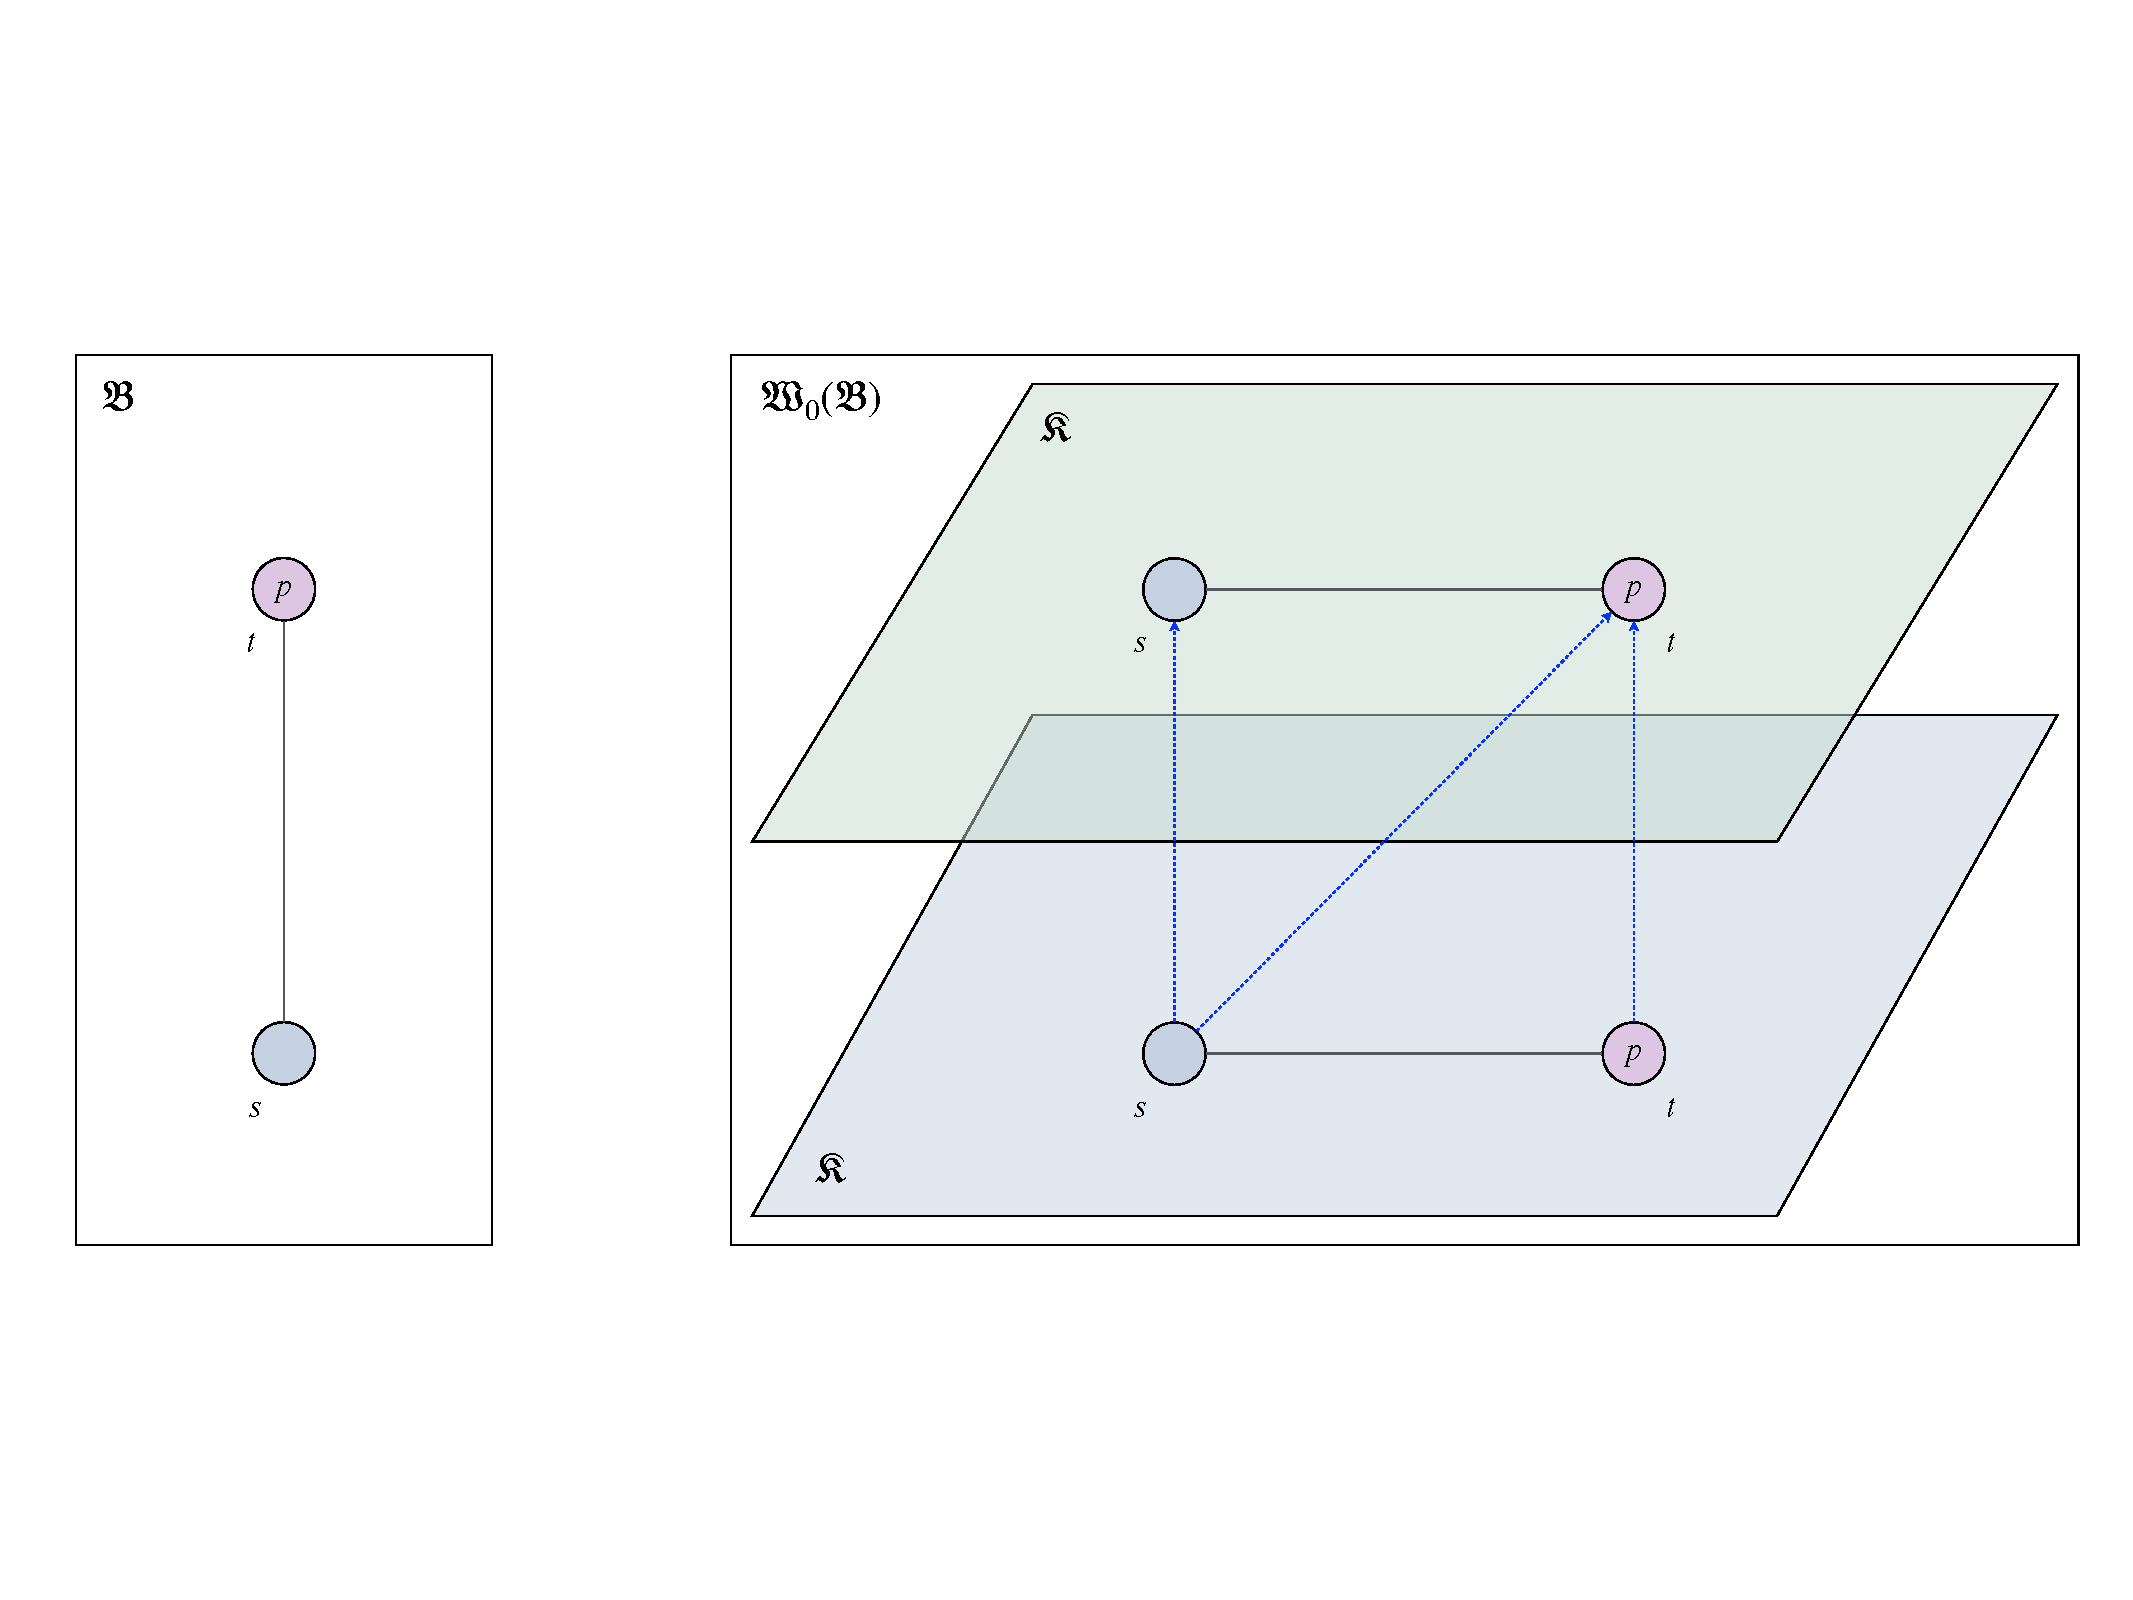
\includegraphics[width=.9\textwidth]{figures/bks2ws.pdf}
  \caption{Bi-relational Kripke model to Weaved model}
  \label{fig:bks2ws}
\end{figure}

\begin{example}
  Let $\bmodel$ be the bi-relational model depicted on the left of \Cref{fig:bks2ws}.
  The model $\wmodel_{\bmodel}$ on the right is the weaved model obtained by applying the construction described in \Cref{prop:bks2ws} to $\bmodel$.
  In $\bmodel$, we are assuming $s \preccurlyeq_{\bmodel} t$.
  This means that $\F_{\wmodel_{\bmodel}}$ contains exactly two relational homomorphisms; i.e.: $\id_{\kmodel}: \kmodel \to \kmodel$ and $f: \kmodel \to \kmodel$ defined as $f(s) = t$ and $f(t) = t$.
  We depicted $f$ with dashed blue lines in \Cref{fig:bks2ws}.
  
  The result in \Cref{prop:bks2ws} also allows us to compare how formulas are evaluated in $\bmodel$ and in the corresponding weaved model $\wmodel_{\bmodel}$.
  In particular, we can verify: ${\bmodel, s \Vdash \Box \lnot \lnot p}$ and $\bmodel, s \nVdash \lnot\lnot\Box p$; and so $\kmodel, s \Vdash^{\wmodel_{\bmodel}} \Box \lnot \lnot p$ and ${\kmodel, s \nVdash^{\wmodel_{\bmodel}} \lnot\lnot\Box p}$.
  We show the side-by-side evaluation of the formula in the models in \Cref{fig:eval}.

  \begin{figure}
    \begin{center}
      \resizebox{\textwidth}{!}{
      \begin{minipage}[t]{.45\textwidth}
        \begin{enumerate}[label=(\alph*),leftmargin=*]
          \item
          $\bmodel, s \Vdash \Box\lnot\lnot p$
          \begin{description}\setlength{\itemsep}{0pt}
            \item[$\bmodel, s \Vdash \Box\lnot\lnot p$]
            \item[for all $\preccurlyeq$] \hfil
            \item[$s \preccurlyeq_{\bmodel} s$] \hfil
              \begin{description}\setlength{\itemsep}{0pt}
                \item[for all $\Box$]
                \item[$s \R_{\bmodel} s$]\hfil
                  \begin{description}
                    \item[$\bmodel, s \Vdash \lnot\lnot p$] 
                    \item[for all $\preccurlyeq$]
                    \item[$s \preccurlyeq_{\bmodel} s$]\hfil
                      \begin{description}
                        \item[$\bmodel, s \nVdash \lnot p$]
                        \item[exists $\preccurlyeq$]
                        \item[$s \preccurlyeq_{\bmodel} t$]\hfil
                          \begin{description}
                            \item[$\bmodel, t \Vdash p$] 
                          \end{description}
                      \end{description}
                    \item[$s \preccurlyeq_{\bmodel} t$]\hfil
                      \begin{description}
                        \item[$\bmodel, t \nVdash \lnot p$]
                        \item[exists $\preccurlyeq$]
                        \item[$t \preccurlyeq_{\bmodel} t$]\hfil
                          \begin{description}
                            \item[$\bmodel, t \Vdash p$] 
                          \end{description}
                      \end{description}
                  \end{description}
                \item[$s \R_{\bmodel} t$]\hfil
                  \begin{description}
                    \item[$\bmodel, t \Vdash \lnot\lnot p$]
                    \item[for all $\preccurlyeq$]
                    \item[$t \preccurlyeq_{\bmodel} t$]\hfil
                      \begin{description}
                        \item[$\bmodel, t \nVdash \lnot p$] 
                      \end{description}
                  \end{description}
              \end{description}
            \item[$s \preccurlyeq_{\bmodel} t$]\hfil
              \begin{description}\setlength{\itemsep}{0pt}
                \item[for all $\Box$]
                \item[$t \R_{\bmodel} s$]\hfil
                  \begin{description}
                    \item[$\bmodel, s \Vdash \lnot\lnot p$]
                  \end{description}
                \item[$t \R_{\bmodel} t$]\hfil
                  \begin{description}
                    \item[$\bmodel, t \Vdash \lnot\lnot p$]
                  \end{description}
              \end{description}
          \end{description}
        \end{enumerate}
      \end{minipage}
      %
      \hfill
      %
      \begin{minipage}[t]{.55\textwidth}
        \begin{enumerate}[label=(\alph*),leftmargin=*]
          \item
          $\kmodel, s \Vdash^{\wmodel_{\bmodel}} \Box\lnot\lnot p$
          \begin{description}\setlength{\itemsep}{0pt}
            \item[$\kmodel, s \Vdash^{\wmodel_{\bmodel}} \Box\lnot\lnot p$]
            \item[for all $\F$] \hfil
            \item[$\id_{\kmodel} : \kmodel \to \kmodel$] \hfil          
              \begin{description}\setlength{\itemsep}{0pt}
                \item[for all $\Box$]
                \item[$\id_{\kmodel}(s) \R_{\kmodel} s$]\hfil
                  \begin{description}
                    \item[$\kmodel, s \Vdash^{\wmodel_{\bmodel}} \lnot\lnot p$] 
                    \item[for all $\F$]
                    \item[$\id_{\kmodel}: \kmodel \to \kmodel$]\hfil                  
                      \begin{description}
                        \item[$\kmodel, \id_{\kmodel}(s) \nVdash^{\wmodel_{\bmodel}} \lnot p$]
                        \item[exists $\F$]
                        \item[$f: \kmodel \to \kmodel$]\hfil                      
                          \begin{description}
                            \item[$\kmodel, f(\id_{\kmodel}(s)) \Vdash^{\wmodel_{\bmodel}} p$] 
                          \end{description}
                      \end{description}
                    \item[$f: \kmodel \to \kmodel$]\hfil
                      \begin{description}
                        \item[$\kmodel, f(s) \nVdash^{\wmodel_{\bmodel}} \lnot p$]
                        \item[exists $\F$]
                        \item[$\id_{\kmodel}:\kmodel \to \kmodel$]\hfil
                          \begin{description}
                            \item[$\kmodel, \id_{\kmodel}(f(s)) \Vdash^{\wmodel_{\bmodel}} p$] 
                          \end{description}
                      \end{description}
                  \end{description}
                \item[$\id_{\kmodel}(s) \R_{\kmodel} t$]\hfil
                  \begin{description}
                    \item[$\kmodel, t \Vdash^{\wmodel_{\bmodel}} \lnot\lnot p$]
                    \item[for all $\F$]
                    {\color{red}
                    \item[$\id_{\kmodel}: \kmodel \to \kmodel$]\hfil
                      \begin{description}
                        \item[$\kmodel, \id_{\kmodel}(t) \nVdash^{\wmodel_{\bmodel}} \lnot p$] 
                      \end{description}
                    \item[$f: \kmodel \to \kmodel$]\hfil
                      \begin{description}
                        \item[$\kmodel, f(t) \nVdash^{\wmodel_{\bmodel}} \lnot p$] 
                      \end{description}
                    }
                  \end{description}
              \end{description}
            \item[$f : \kmodel \to \kmodel$]\hfil
              \begin{description}\setlength{\itemsep}{0pt}
                \item[for all $\Box$]
                \item[$f(s) \R_{\kmodel} s$]\hfil
                  \begin{description}
                    \item[$\kmodel, s \Vdash^{\wmodel_{\bmodel}} \lnot\lnot p$]
                  \end{description}
                \item[$f(s) \R_{\kmodel} t$]\hfil
                  \begin{description}
                    \item[$\kmodel, t \Vdash^{\wmodel_{\bmodel}} \lnot\lnot p$]
                  \end{description}
              \end{description}
          \end{description}
        \end{enumerate}
      \end{minipage}
      }
    \end{center}
    \caption{Side-by-side Evaluation}\label{fig:eval}
  \end{figure}
  
\end{example}